\documentclass[UTF8]{ctexart}
\usepackage{mathtools,wallpaper}
\usepackage{t1enc}
\usepackage{pagecolor}
\usepackage{enumitem}
\usepackage{hyperref}
\usepackage{graphicx}
\usepackage{listings}
\usepackage{amssymb}
\usepackage[dvipsnames]{xcolor}
\usepackage{float}
\usepackage{numerica}



\begin{document}

\section{Sets, Relations and Languages}

\subsection{Sets}
\begin{itemize}
    \item Set notion
    \begin{enumerate}
        \item Enumeration method
            For example, \(A={1,2,3}\) ,or \(N={0,1,2, ...}\)
        \item Descriptive method
            For example, the set of odd natural numbers is \(O=\{x: x \in N\) and x is not divisible by 2\}.
        \item Singleton
            Singleton set contains only one element.
        \item Empty Set
            $\phi$ 
        \item 集合中的元素之间可以没有任何关系
        \item Sets have Reciprocity（互异性），\{1, 2, 3\} and \{1, 1, 2, 3\} 是相同的集合。
        \item The set does not distinguish the order of the elements. So, two sets are the same if and only if they have the same elements.
    \end{enumerate}
    \item 子集和真子集
    
        If every element of set A is an element of set B, then A is said to be a subset of B, $A \subseteq B$.

        If A is a subset of B but A is not the same as B, so A is a proper subset of B and write $ A \subset B$.  
    
    \item Set operations
    \begin{enumerate}
        \item Intersection $A \cap B = \{x, x\in A \text{ and } x \in B\}$. 
        
        A=\{1,3,9\}, B=\{3,5,7\}, $A \cap B$=\{3\}
        \item Union $A \cup B = \{x, x \in A \text{ or } x \in B\}$
        \item The difference of two sets $A-B=\{x, x \in A \text{ and } x \notin B\}$
        \item Idempotency幂等律: $A \cap A = A$, $A \cup A = A$
        \item Commutativity交换律: $A \cup B = B \cup A$, $A \cap B = B \cap A$
        \item Associativity结合律: $(A \cup B) \cup C = A \cup (B \cup C)$, $(A \cap B) \cap C = A \cap (B \cap C)$
        \item Distributivity分配律: $(A \cup B) \cap C = (A \cap B) \cup (A \cap C)$, $(A \cap B) \cup C = (A \cup B) \cap (A \cup C)$
        \item Absorption吸收率: $(A \cap B) \cup A = A$, $(A \cup B) \cap A = A$
        \item DeMorgan's laws德摩根定律: $A-(B \cap C) = (A-B) \cup (A-C) $, $A-(B \cup C) = (A-B) \cap (A-C) $
    \end{enumerate}

    \item 证明DeMorgan's laws德摩根定律: $A-(B \cap C) = (A-B) \cup (A-C) $
    
    Using the theorem, two sets are the same if and only if they have the same elements. We must prove $L \subseteq R $ and $R \subseteq L$.
    Let $L=A-(B \cap C)$, $ R= (A-B) \cup (A-C)$. 

    Firstly, let x be any element of L; then $x \in A$, but $x \notin B$ and $x \notin C$. Hence x is an element of A-B and A-C,and x is thus an element of R, therefore $L \subseteq R$.

    Secondly, let x be any element of R; then x is both in $x \in (A-B)$ and $x \in (A-C)$, and x is therefore in A but in neither B or C. Hence $x \in A$ but $x \notin B \cup C$, so $x \in L$. Therefore $R \subseteq L$.

    \item binary operation of the Set
    
    $\cup S=\{x:x \in P \text{ for some set } P \in S \}$ 

    $\cap S=\{x:x \in P \text{ for each set } P \in S \}$ 

    For example, $S=\{\{a,b\},\{b,c\},\{c,d\}\}$,$\{a,b\}\cup\{b,c\}\cup\{c,d\}=\{a,b,c,d\}$=$\cup S$,

    \item A的幂集
    
    The power set of A，denoted $2^A$, is the collection of all subsets of a set of A. 
    
    eg: $2^{\{c,d\}} =\{\{c,d\},\{c\},\{d\},\phi\}$.

    \item Partition of a Set
    
    一个非空集合A的Partition是其幂集$2^A$的子集$\varPi$,并且在$\varPi$中不包括$\phi$，每一个A中的元素都只在$\varPi$中一个集合。
    
    $\varPi$ is a partition of A if $\varPi$ is a set of subset of A, such that

    (1)each element of $\varPi$ is nonempty

    (2)distinct members of $\varPi$ are disjoint

    (3)$\cup \varPi$ is A

    
\end{itemize}

\subsection{Relations and Functions}
\begin{itemize}
    \item 有序对
    
    Ordered pairs represent the relationship between objects. In the ordered pair (a,b), a and b are the components, and (a,b) is not the same as (b,a).

    \item Cartesian product(笛卡尔积)
    
    The Cartesian product of two sets A and B, denoted by AxB, is the set of ordered pairs (a,b) with $a \in A$ and $b \in B$.
    
    两集合上的二元关系(denoted by Q)，就是它们笛卡尔积的任意子集。A binary relation on two sets A and B are sets of ordered pairs (a, b) of any $a \in A$ and $b \in B$.

    \item n-ary relation(n元关系)
    
    如果$A_1,A_2,...,A_n$是任一集合，这些集合的n折笛卡尔积是所有有序n元组的集合(a1,a2,..,an).

    An ordered m-tuple(b1,...,bm) is the same as (a1,..,an) if and only if m=n and ai=bi, for i=1,...,n

    \item Functions
    \begin{enumerate}
        \item 定义：A function is an association of each object of one kind with unique object of another kind.
        
        \item $f:A\rightarrow B$ indicate f is the function from A to B, where A is the domain of f and b is the range of f. If $a \in A $, $f(a)$ is the image(像) of a under f.
        
        \item 从集合A到集合B的函数是一个在A和B上的关系R，for each element $a \in A$ there is an exactly one ordered pair in R with first component a.
        
        \item 单射, $f:A \rightarrow B$ is one-to-one if for any two distinct elements $a,a^{'} \in A$,$f(a)\neq f(a^{'})$.
        \item 满射, $f:A \rightarrow B$ is onto B, if each element of B is the image under f of some elements of A.
        \item 双射, $f:A \rightarrow B$ is bijection between A and B if both one-to-one and onto B.
    \end{enumerate}

\subsection{Special types of Binary Relations}



\end{itemize}
Node can be represented by the element of set, arrow is the relation direction, then node and arrow can construct directed/undirected graph.

\begin{itemize}
    \item 自反关系
    
    A relation $R \subseteq A*A$ is reflexive if $(a,a) \in R$ and $a \in A$.在有向图，一个自反关系表示每个节点都有一条指向自身的环。
    \item 对称关系
    
    A relation $R \subseteq A*A$ is symmetric if $(a,b) \in R$ whenever $(b,a) \in R$.在有向图中表示两个节点一定有双向箭头。

    如果有向图满足对称关系，那么将来回箭头合并为直线。
    \item 反对称关系
    
    A relation R is antisymmetric if whenever $(a,b) \in R$ and a and b are distinct, then $(b,a) \notin R$. 可以有环，但是不同的元素不能有双向关系，请注意(a,a)是反对称的。

    \item 传递性
    
    A binary relation is transitive if whenever $(a,b) \in R$ and $(b,c) \in R$, then $(a,c) \in R$.

    \item 等价关系
    
    An equivalence relation is a relation that is reflexive, symmetric, transitive. 

    等价关系由包含很多cluster(簇)的无向图表示，等价关系中的簇又被称为等价类。

    簇：等价关系可以划分出簇，不同的簇不能有交集，所有簇的并集应等于原集合。

    等价类是一个集合，已知等价关系，我们用$[a]$表示包含元素a的等价类关系，$[a] =\{b: (a, b) \in R\}$.


\end{itemize}

\subsubsection{Theorem}
Let R be an equivalence relation on a nonempty set A. Then the equivalence classes of R can constitute the partition of A.

根据划分和等价类的定义，我们需要证明由$[a]$组成的等价类集合是非空，其中自己互斥并且所有子集的并集是原集合。这里我们使用数学中的反证法。

By reflexive, $(a,a) \in R $, $a \in [a] $, $a \in A$, all equivalence classes are nonempty.

To show that they are disjoint, consider any two distinct equivalence classes [a] and [b], and suppose that $[a] \cap [b] \neq \varnothing $. Thus there is an element c, $c \in [a]$ and $c \in [b]$. Hence in equivalence relation, $(a,c) \in R$ and $(c,b) \in R$, and $(a,b) \in R$ by transitivity; and since symmetric in R, $(b,a) \in R$. For any element $d \in [a]$, $(d,a) \in [a]$; by transitivity $(d,b) \in [b]$; hence $d \in [b]$. Hence $[a] \subseteq [b]$. Likewise $[b] \subseteq [a]$. Therefore [a]=[b]. But this contradicts the assumption that [a] and [b] are distinct. So $[a] \cap [b] = \varnothing$.

Each element a of A is in $\varPi$ by reflexive of $R$.

\begin{itemize}
    \item partial order(偏序关系)
    
    \begin{enumerate}
        \item Partial order is a relation that is reflexive, antisymmetric and transitive.
        \item 全序关系，a partial order $R \subseteq A*A$ is a total order, if for all $a,b \in A$, either (a,b) or (b,a) $\in R$.
        \item 全序关系需要任意两个元素都能够被比较。
    \end{enumerate}

    \item Path: A path in a binary relation $R \subseteq A*A$ is a sequence$(a_1,...,a_n)$.
    \item Cycle: The path $(a_1, ... , a_n) \text{ is a cycle if the } a_i \text{'s are all distinct and also } (a_n, a_1) \in R.$

\end{itemize}

\subsection{Finite and Infinite Sets有限集和无限集}

\begin{itemize}
    \item 有限集的基本属性是size，即集合包含元素的数量。
    \item equinumerous(等势).Two sets A and B are equinumerous if there is a bijection $f:A \rightarrow B$.
    \begin{enumerate}
        \item If a set is equinumerous with the natural number set\{1,2,...,n\}(n是一个确定的数值); the set is finite set and the cardinality of the set is n. In summary, The cardinality of finite set is the number of the elements in it.
    \end{enumerate}
    \item infinite set无限集
    \begin{enumerate}
        \item 如果一个集合不是有限集，那么就是无限集。
        \item 如果一个无限集与自然数集N等势，即无限集中每一个数都能够与自然数集中每一个数对应，则称无限集为可数无限集。
        \item Dovetailing(交织法) can prove that the union of a countably infinite collection of countably infinite sets is countably infinite. A = \{a0, a1, ... \}, B = \{b0, b1, ... \} ,C = \{ c0, c1 , ... \} , Then their union can be listed as $A \cup B \cup C$ = \{a0, b0, c0, a1, b1, c1 ,a2, ...\} 
        \item N is natural number set, show N*N is countably infinite.(使用了康托尔配对函数)
        
        在第0层，有一对(0,0);在第1层，有两对(1,0)(0,1);在第2层，有三对(0,2)(1,1)(2,0);在第w-1层，(0,w-1)(1,w-2)...(w-1,0),从0到w-1，一共有w对。
        所以在w层之前，我们一共有
        \begin{equation}
            \begin{aligned}
                1+2+3+...+w &= \frac{w(1+w)}{2}
            \end{aligned}
        \end{equation}

        $w=i+j$,(i,j)。在第w层，i表示在这一层第i个被访问的。
        总序号$m=\frac{w(1+w)}{2}+i$    
        得到康托尔配对标准式子$m=\frac{(i+j)(i+j+1)}{2}+i$  

        因此我们可以将N*N与自然数集N进行双射。N*N是一个可数无限集。
    \end{enumerate}
\end{itemize}

\subsection{Mathematics Proof Technique}
\begin{itemize}
    \item Mathematical induction 
    
    数学归纳法一般用来证明给定命题在自然数的整个或者部分范围是正确的。

    数学归纳法的原理，首先证明该命题在某个起始值是成立的，然后证明从一个值到下一个值的过程也是成立的。当这两点都证明成立后，反复使用这种方法，就能推导出任何值的情况。

    \begin{figure}[h]
        \centering
        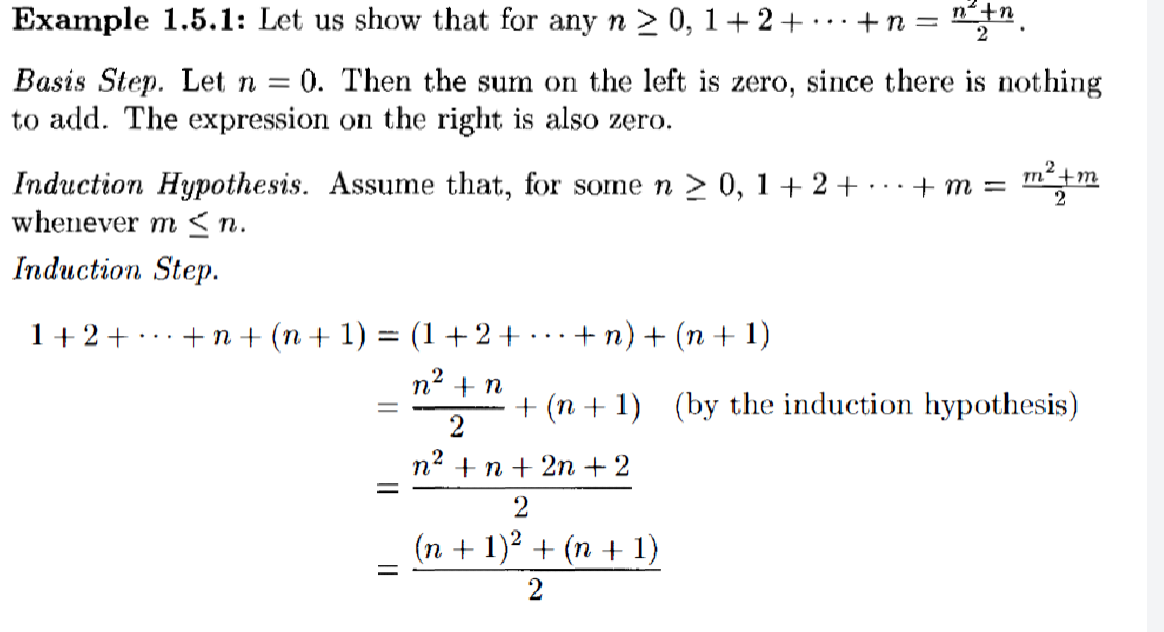
\includegraphics[width=1\textwidth]{static/Mathematical-induction.png}
        \caption{Mathematical-induction} 
        \label{Mathematical-induction}
    \end{figure}

    \item Pigeonhole Principle(鸽巢原理)
    若A和B是有限集，$|A|>|B|$，则不存在从A到B一一对应的函数。

    \begin{figure}[H]
        \centering
        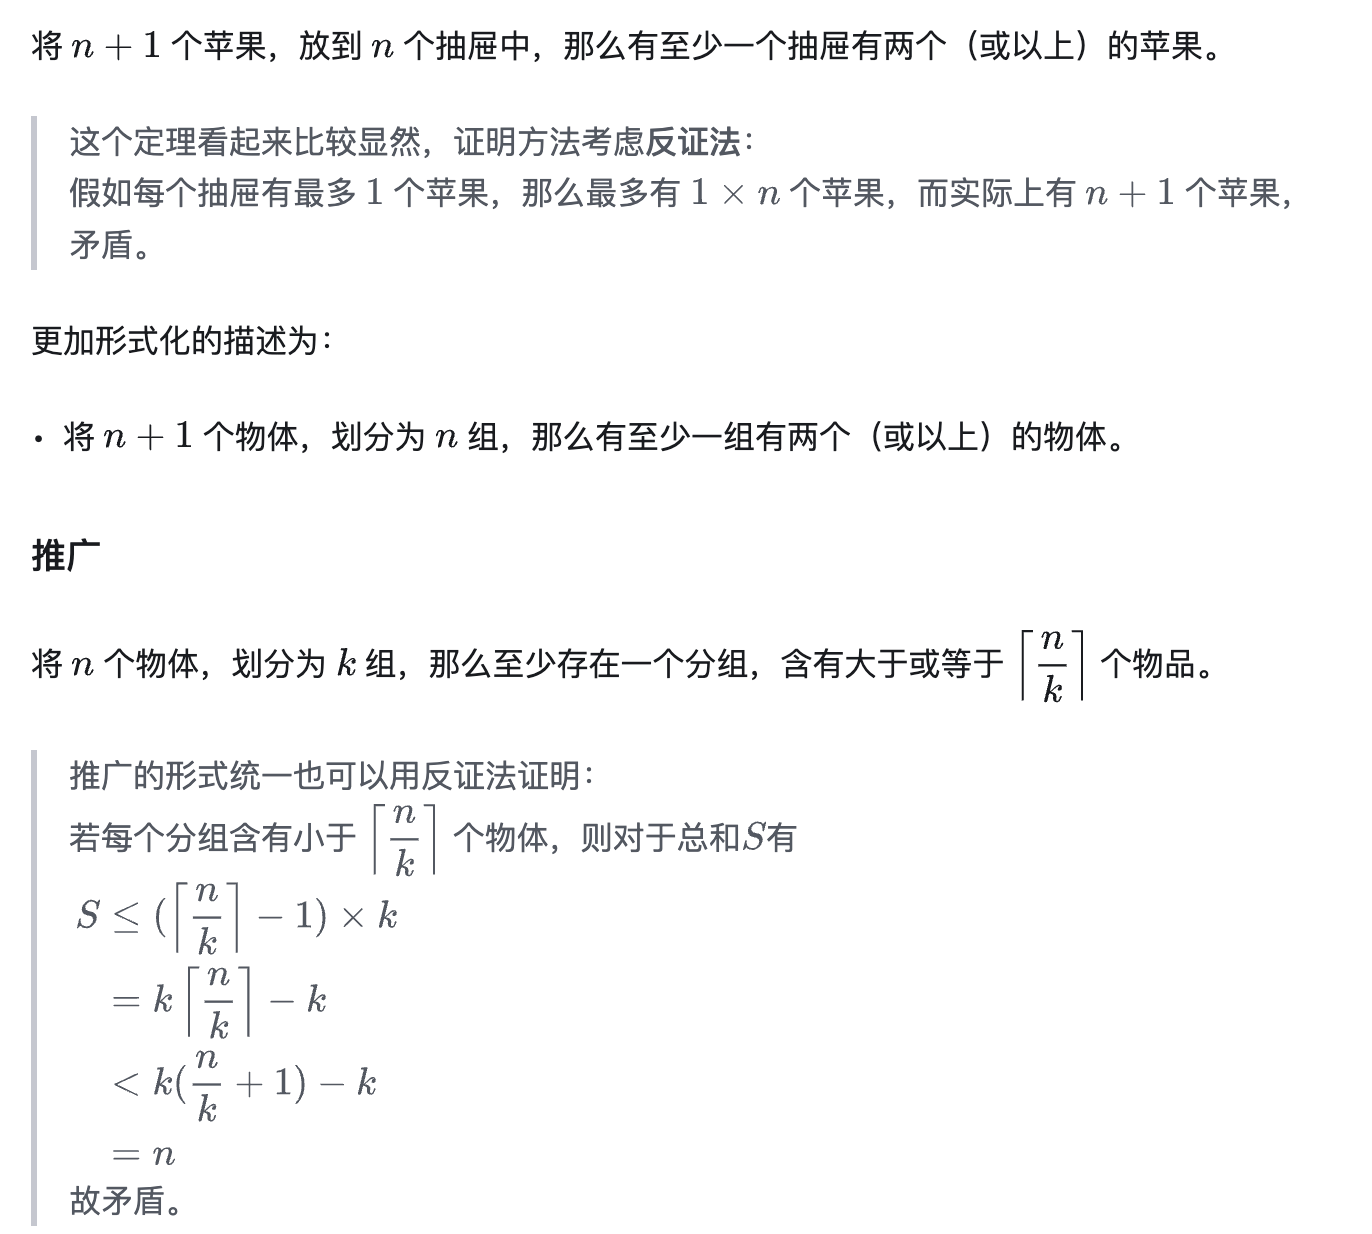
\includegraphics[width=1\textwidth]{static/Pigeonhole-Principle1.png}
        \caption{Pigeonhole-Principle1} 
        \label{Pigeonhole-Principle1}
    \end{figure}

    \begin{figure}[H]
        \centering
        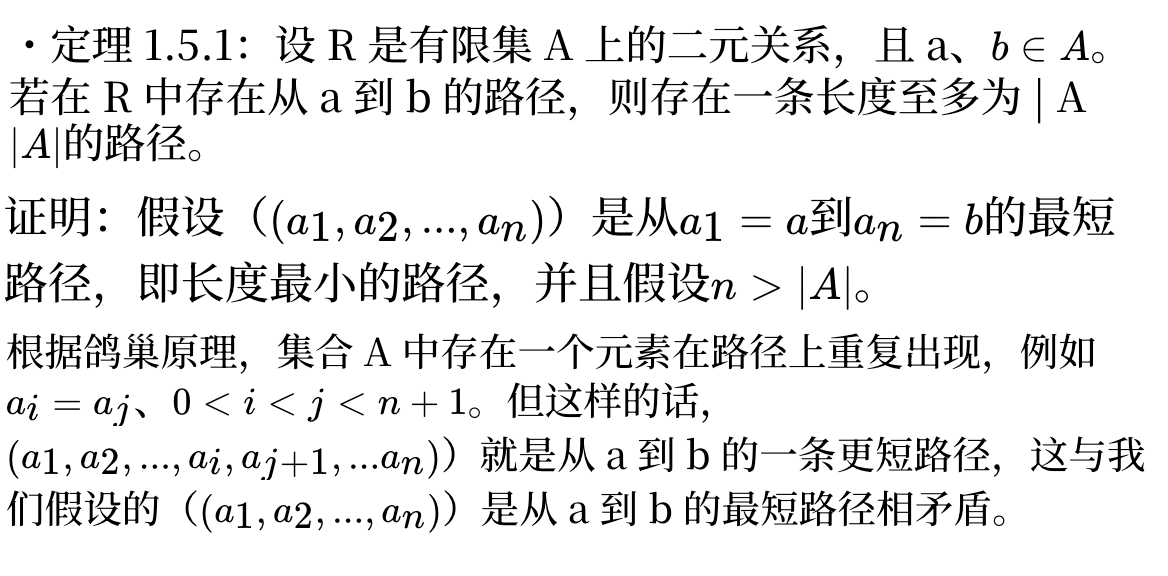
\includegraphics[width=0.7\textwidth]{static/Pigeonhole-Principle2.png}
        \caption{Pigeonhole-Principle2} 
        \label{Pigeonhole-Principle2}
    \end{figure}

    \item Diagonalization Principle(对角化理论)
    
    R是集合A的二元关系，设D是R的对角集(Diagonalization set),
    $D=\{a:a \in A \text{ and } (a,a) \notin R\}$; 
    
    for each $a \in A$, define $R_a=\{b:b \in A \text{ and } (a,b) \in R\}$,$R_a$是行集，即所有与a有关系R的元素集合。

    由此我们可以发现，对于diagonal set D，如果element a存在reflexive relation，那我们不将其加入D集合中，若没有自反关系，我们加入对角集，即我们取主对角线的补集。$R_a$对应数组的每一行，对于元素为a的行，取b(b可以和a相等)。

    \item eg：The set $2^N$ is uncountable.

    Supposing $2^N$ is countable infinite set, there is a way of enumerating all members of $2^N=\{R_0,R_1,R_2,...\}$,$R_i$ is $R_a$ in the statement of diagonalization principle.
    Consider an diagonal set $D=\{n \in N:n \notin R_n\}$. D is a set of natural number, D should be in $R_n$,n = 1,2,...。But according to diagonalization principle, D can not appear in $R_n$, then it is a contradiction.

    So,the set $2^N$ is uncountable.

\end{itemize}

\subsection{Closures and Algorithm}
\begin{itemize}
    \item 自反传递闭包
    \begin{enumerate}
        \item Let \(R \subseteq A^{2}\) be a directed graph defined on a set \(A\). The \textbf{reflexive transitive closure} of \(R\) is the relation 
        \[
        R^{*} = \{(a, b) \mid a, b \in A \text{ and there is a path from } a \text{ to } b \text{ in } R\},
        \] 
        and \(R^{*}\) is reflexive. \(R^{*}\)是包含R并且同时满足自反和传递的最小关系。

        \item 算法
        \begin{figure}[H]
            \centering
            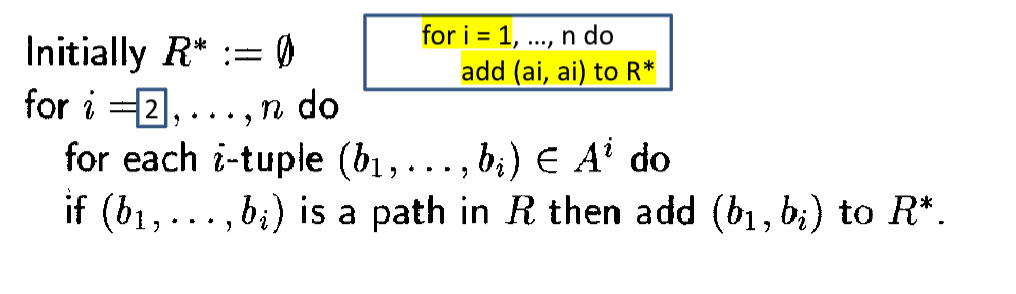
\includegraphics[width=1\textwidth]{static/reflexive-transitive-closure.png}
            \caption{reflexive-transitive-closure} 
            \label{reflexive-transitive-closure}
        \end{figure}
    \end{enumerate}
    
    \item 闭包算法定义
    
    \begin{enumerate}
        \item Let $D$ be a set, let $n \geq 0$, and let $R \subseteq D^{n+1}$ be a $(n+1)$-ary relation on $D$. 
                Then a subset $B$ of $D$ is said to be \textbf{closed under $R$} if $b_{n+1} \in B$ whenever
                $b_1, \ldots, b_n \in B$ and $(b_1, \ldots, b_n, b_{n+1}) \in R$.

                R是D的n+1元关系，如果通过输入B，将$b_1$到$b_n$通过关系R输出得到$b_{n+1}$,那么$b_{n+1}$也属于B。
        \item 闭包从一个较大的集合D和D的子集A开始，构建包含A且满足闭包性质的最小集合B。
        \item (1)B contains A ；(2)B is the minimal set containing A and A and closed under \(R_{1}\) , \(R_{2}, ... R_{m}\)
    \end{enumerate}

\end{itemize}

\subsection{Alphabets and Languages字母表和语言}
\begin{itemize}
        \item \textbf{Alphabet}: Finite set of symbols (e.g., $\{0, 1\}$).
        \item \textbf{String}: Finite sequence of symbols from an alphabet.
        \item \textbf{Empty string}: String with no symbols, denoted $e$.
        \item \textbf{Length}: $|w|$ = number of symbols in string $w$; $|e| = 0$.
        \item \textbf{Indexing}: $w(j)$ = symbol at position $j$ in string $w$.下标从1计算。
        
        \item String Operation
        \begin{enumerate}
            \item String concatenation, denoted by $x \circ y$ or $xy$. x is the prefix of w, y is the suffix of w.
            $w = x \circ y$ if and only if:
            
            $|w| = |x| + |y|$,
            
            $w(j) = x(j)$ for all $j = 1, \dots, |x|$,
            
            $w(|x| + j) = y(j)$ for all $j = 1, \dots, |y|$.

            \item For each string $w$ and each natural number $i$, the string $w^{i}$ is defined recursively as:
            \[w^{0} = \varepsilon,\]
            \[w^{i+1} = w^{i} \circ w, \quad \text{for each } i \geq 0.\]

            \item 字符串反转reversal of string
            
            The reversal of a string w, denoted by \(w^{R}\).
            Details as follows：
            (1)If w is a string of length 0, then $w_R=w=e$.
            (2)If w is a string of length n+1>0, then w=ua for
            some $a \in \sum $, and $w^R=au^R$.

            \begin{figure}[H]
                \centering
                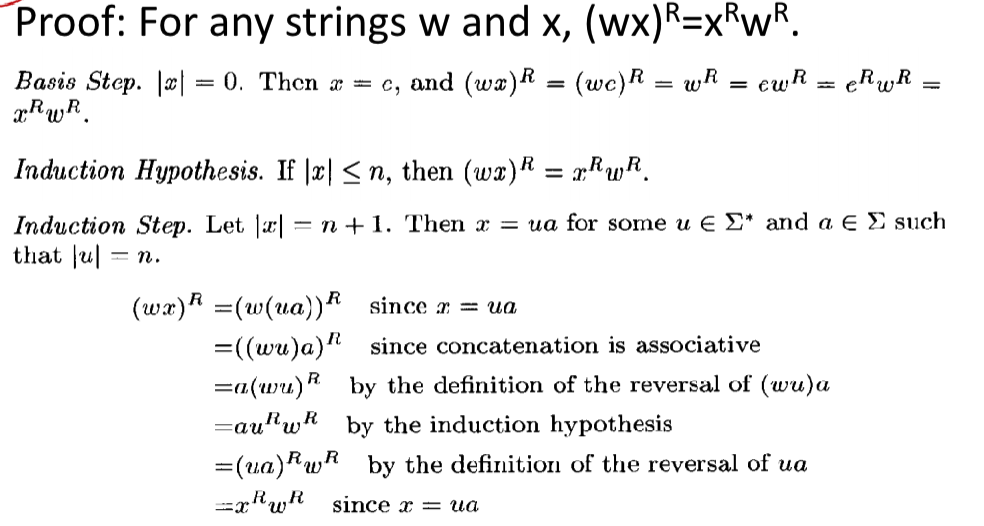
\includegraphics[width=0.7\textwidth]{static/string-reverse.png}
                \caption{string-reverse} 
                \label{string-reverse}
            \end{figure}

        \end{enumerate}
        \item infinite strings
        \begin{enumerate}
            \item 字母表$\sum $中字符组成的所有字符串包括空字符串在内的字符串记作$\sum^* $.
            \item language: Any set of strings over an alphabet$\sum$, or any subset of $\sum^* $.
            \item 语言是一个集合，包含的元素数量可以是无限的。我们使用式子来定义语言：$L=\{w \in \sum^*, \text{w has property P}\}$.
            \item Proof$\sum^*$ is a countably infinite set？
            \begin{figure}[H]
                \centering
                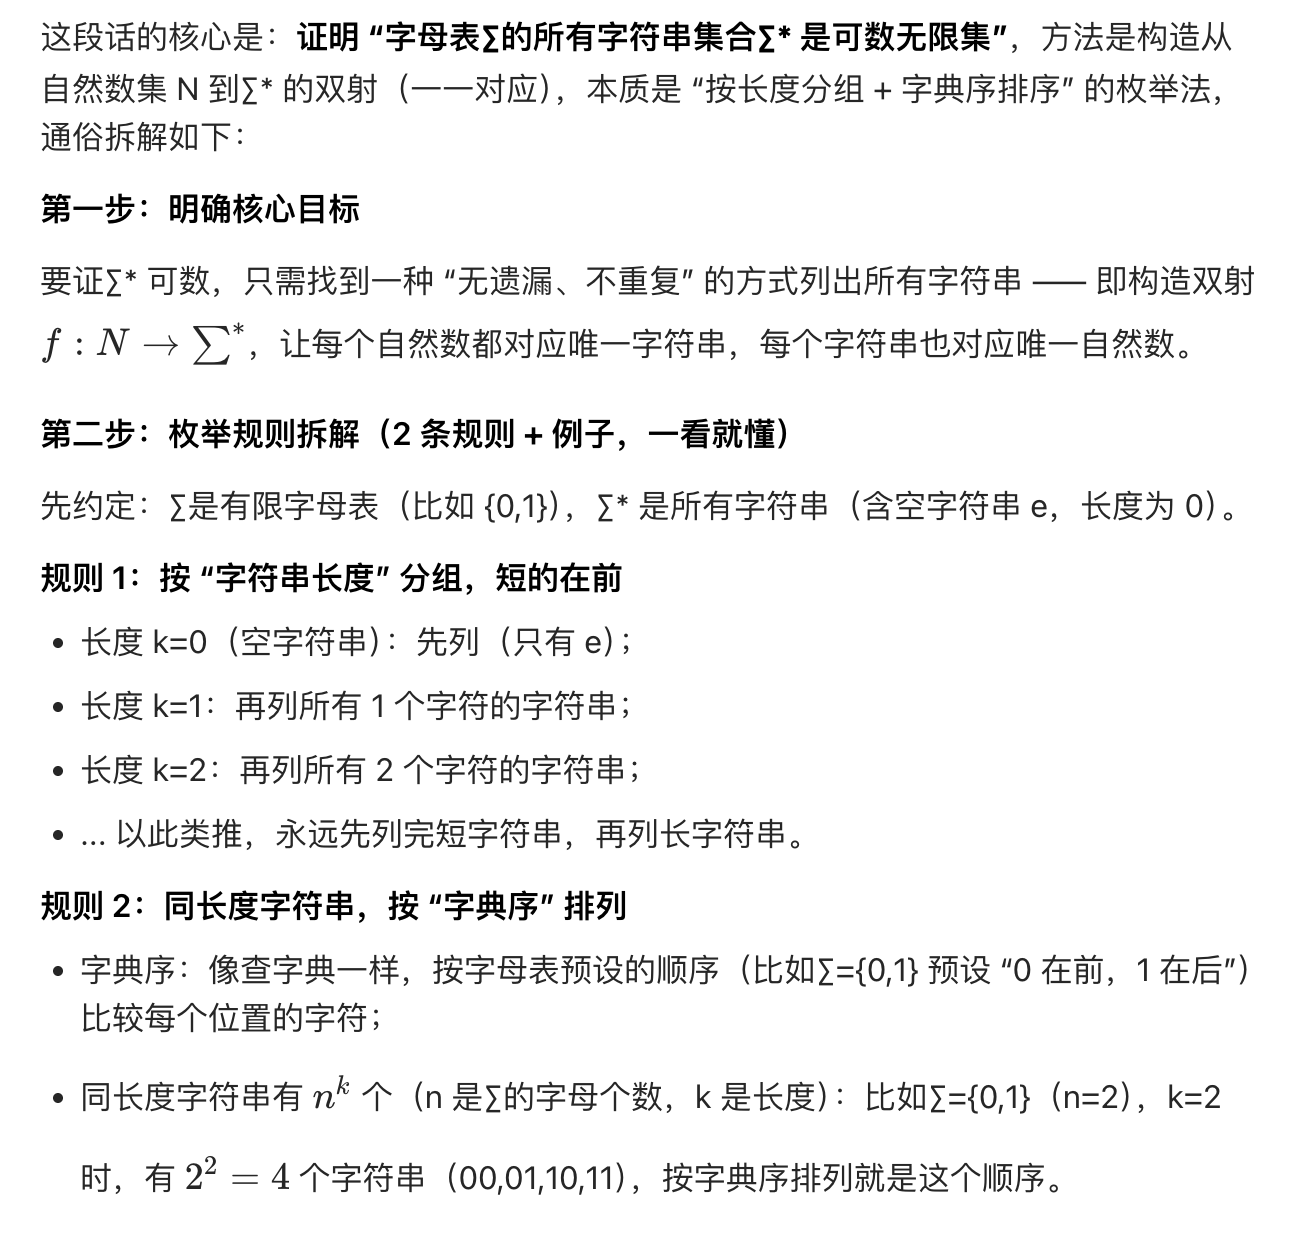
\includegraphics[width=0.7\textwidth]{static/countably-language-set.png}
                \caption{countably-language-set} 
                \label{countably-language-set}
            \end{figure}
            \item Operations on Languages

            Languages can be combined using set operations to define new languages.
            例如，$\overline{A}$ 表示 $A$ 的补集，定义为 $\overline{A} = \Sigma^{*} - A$。

            \item The Concatenation of Languages
            Let $L_1, L_2 \subseteq \Sigma^{*}$ be languages over alphabet $\Sigma$. 
            The \emph{concatenation} of $L_1$ and $L_2$, denoted $L_1 L_2$ or $L_1 \circ L_2$, 
            is defined as:
            \[
            L_1 L_2 = \{ w \in \Sigma^{*} : w=x\circ y, \text{ for some } x \in L1, y \in L2 \}.
            \]

            \item Kleene stare denoted $L^*$. $L^*$是通过连接L中0个或多个字符串得到的所有字符串的集合。
        \end{enumerate}

\end{itemize}

\subsection{Finite Representations of Languages语言的有限表示}
可数有限或者可数无限语言能够使用语言的有限表示进行表示，比如正则表达式，不可数无限语言不能使用有限表示进行表示。
\begin{figure}[H]
    \centering
    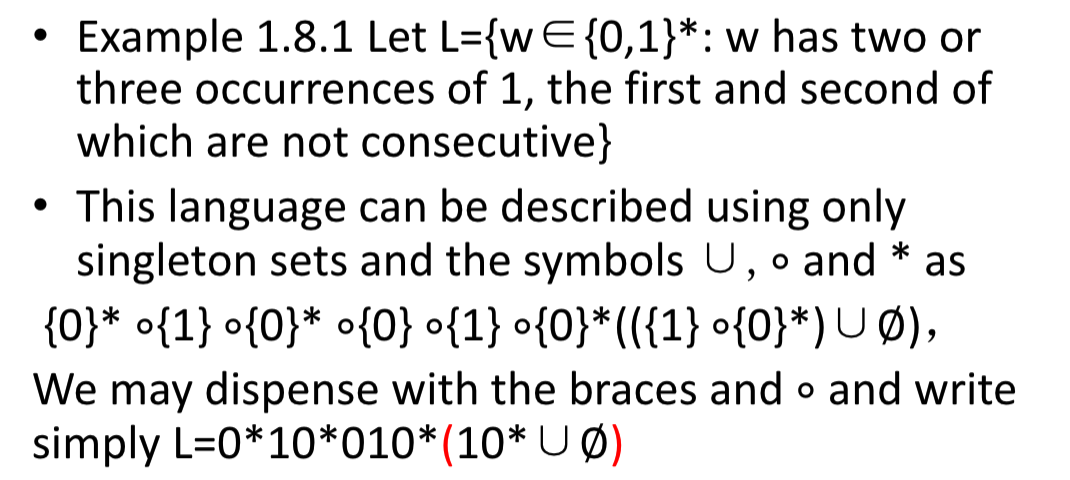
\includegraphics[width=1\textwidth]{static/two-or-three-occurrences1.png}
    \caption{two-or-three-occurrences1} 
    \label{two-or-three-occurrences1}
\end{figure}

\begin{itemize}
    \item regular expression
    \begin{enumerate}
        \item \textbf{语义函数 $L$}：
        设 $a$ 是正则表达式，则 $L(a)$ 表示 $a$ 所描述的语言。函数 $L$ 从正则表达式映射到语言。
        
        \item \textbf{基础定义 (Base Cases)}：
        \[
        L(\emptyset) = \emptyset, \quad L(a) = \{a\} \quad \text{对每个 } a \in \Sigma
        \]
        其中 $\emptyset$ 表示空集（不接受任何字符串），$\{a\}$ 表示只包含单个字符 $a$ 的语言。
        \begin{figure}[H]
            \centering
            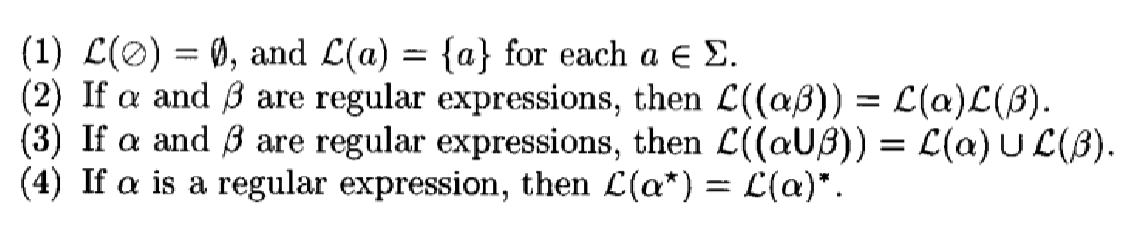
\includegraphics[width=1\textwidth]{static/RegularExpression-BaseCases.png}
            \caption{RegularExpression-BaseCases} 
            \label{RegularExpression-BaseCases}
        \end{figure}
        
        \item \textbf{递归构造 (Recursive Construction)}：
        若 $\alpha$ 和 $\beta$ 是正则表达式，则：
        \begin{itemize}
            \item \textbf{连接 (Concatenation)}：
            \[
            L((\alpha \beta)) = L(\alpha) \circ L(\beta)
            \]
            \item \textbf{并 (Union)}：
            \[
            L((\alpha \cup \beta)) = L(\alpha) \cup L(\beta)
            \]
            \item \textbf{Kleene 星 (Kleene Star)}：
            \[
            L(\alpha^{*}) = L(\alpha)^{*}
            \]
        \end{itemize}
        \begin{figure}[H]
            \centering
            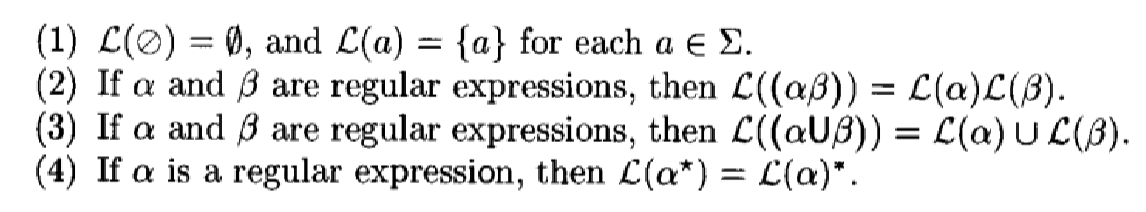
\includegraphics[width=1\textwidth]{static/RegularExpression-operation.png}
            \caption{RegularExpression-operation} 
            \label{RegularExpression-operation}
        \end{figure}

        \begin{figure}[H]
            \centering
            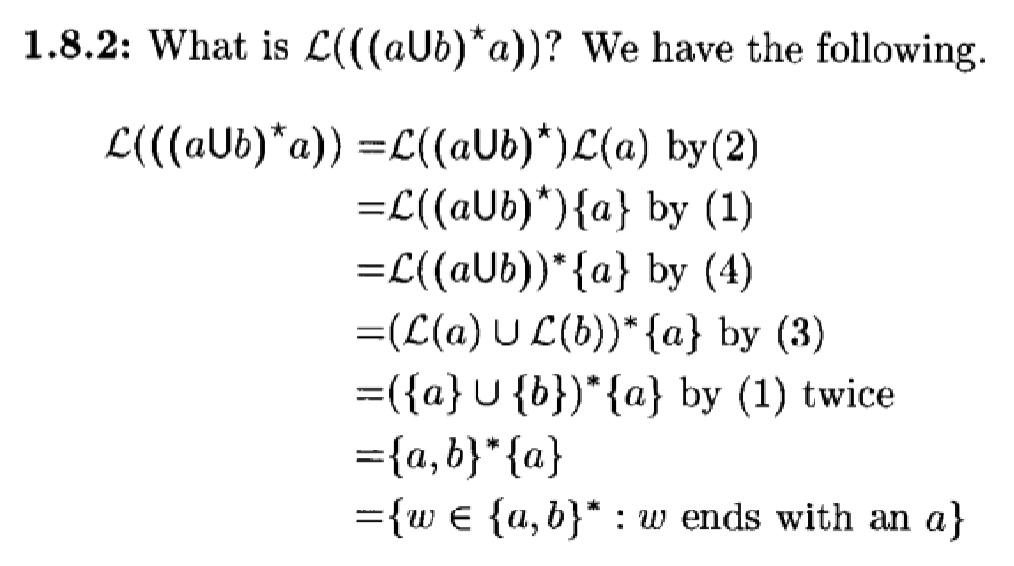
\includegraphics[width=1\textwidth]{static/RegularExpression-operation-eg.png}
            \caption{RegularExpression-operation-eg} 
            \label{RegularExpression-operation-eg}
        \end{figure}
        
        \item \textbf{正则语言 (Regular Languages)}：
        字母表 $\Sigma$ 上的正则语言类定义为：
        \[
        \{ L \subseteq \Sigma^{*} \mid L = L(a) \text{ 对某个正则表达式 } a \}
        \]
        即：正则语言是能用正则表达式描述的所有语言。
        
        \item \textbf{闭包刻画 (Characterization via Closure)}：
        正则语言类是集合
        \[
        \{ \{w\} \mid w \in \Sigma^{*} \} \cup \{\emptyset\}
        \]
        在并、连接和 Kleene 星运算下的闭包。

        \item 问题
        但是对于一些情况，我们还是没法使用正则表达式进行表示。
    \end{enumerate}
    
    
    
    \item language generator
    
    Language generator describe how a generic specimen in the language is produced
    \begin{figure}[H]
        \centering
        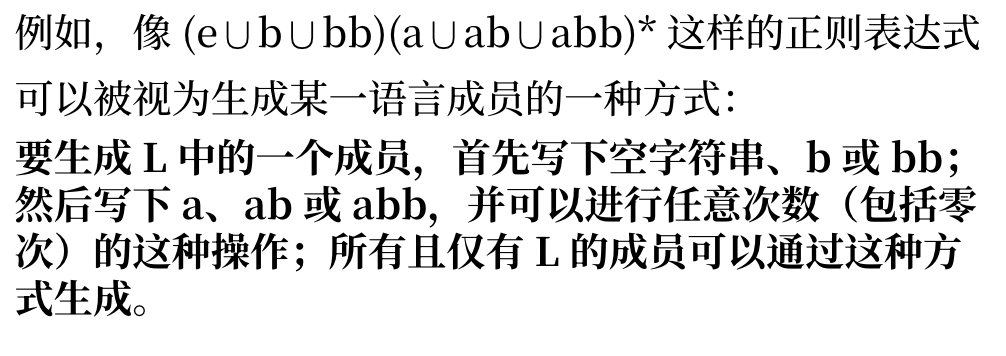
\includegraphics[width=1\textwidth]{static/language-generator.png}
        \caption{language-generator} 
        \label{language-generator}
    \end{figure}

    \item language recognition device
    
        \textbf{定义}: 专门为某个语言 $L$ 设计的算法，用于回答形如“字符串 $w$ 是否属于 $L$？”的问题，称为该语言的\textbf{语言识别装置}。
    
        \textbf{关键要求}: 必须存在算法能确定任意给定字符串是否属于该语言。
    \begin{figure}[H]
        \centering
        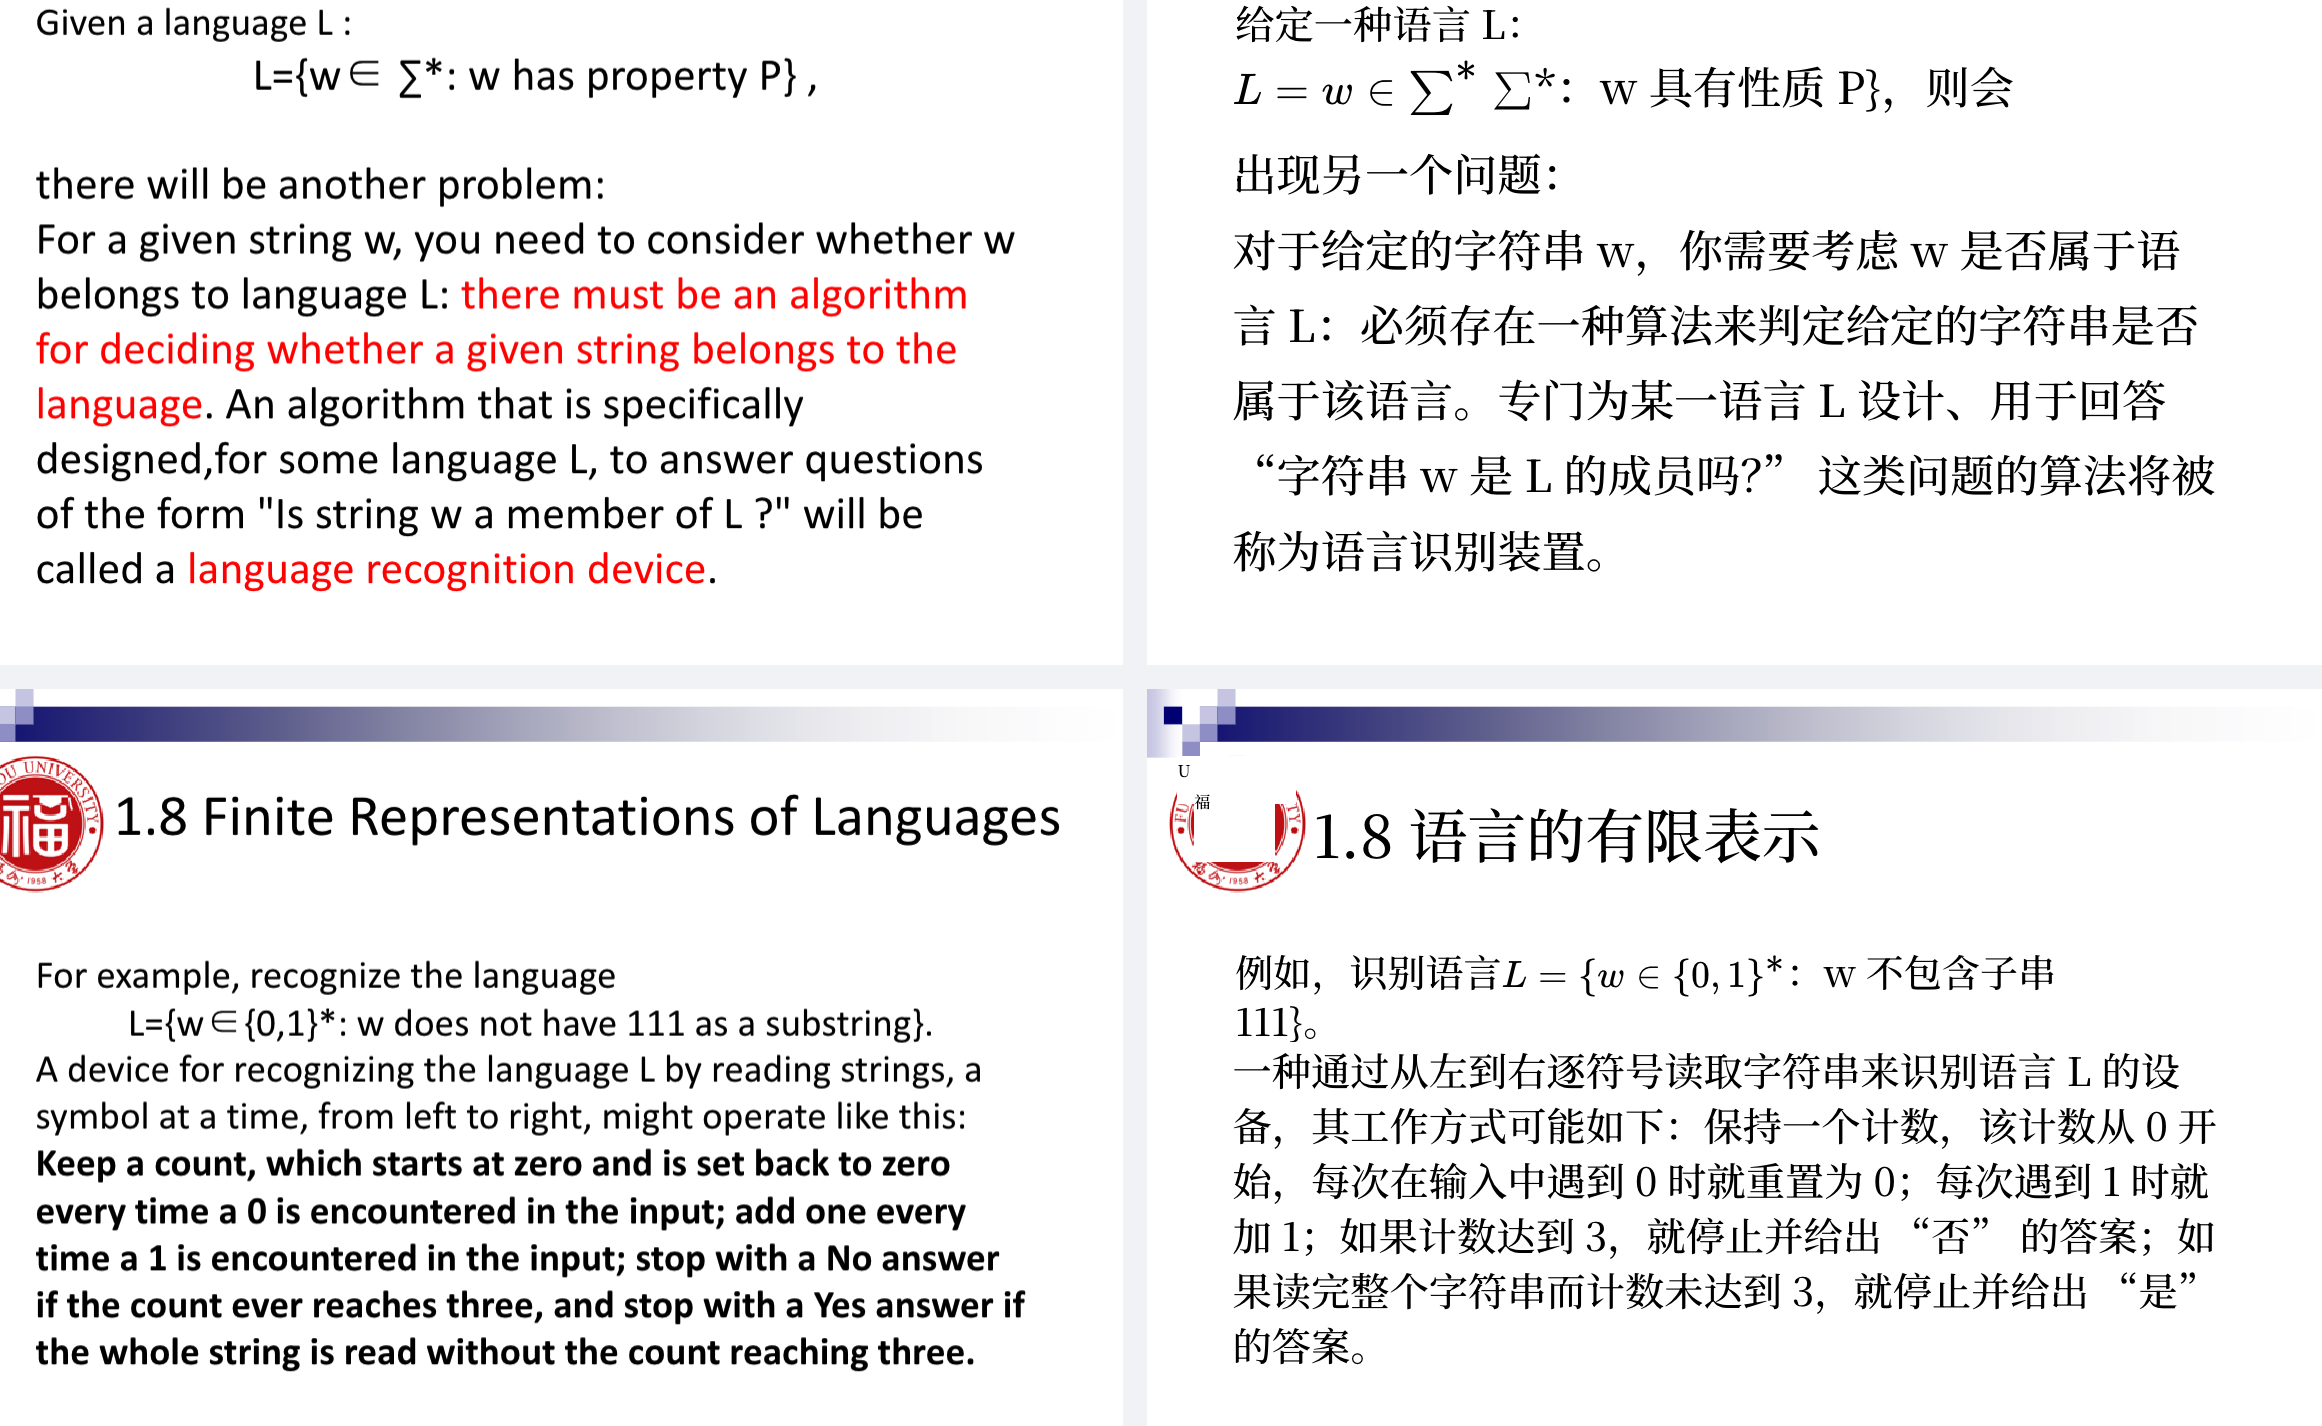
\includegraphics[width=1\textwidth]{static/language-recognition-device.png}
        \caption{language-recognition-device} 
        \label{language-recognition-device}
    \end{figure}
\end{itemize}

\end{document}